\iffalse
\let\negthickspace\undefined
\documentclass[journal,12pt,twocolumn]{IEEEtran}
\usepackage{cite}
\usepackage{amsmath,amssymb,amsfonts,amsthm}
\usepackage{algorithmic}
\usepackage{graphicx}
\usepackage{textcomp}
\usepackage{xcolor}
\usepackage{txfonts}
\usepackage{listings}
\usepackage{enumitem}
\usepackage{mathtools}
\usepackage{gensymb}
\usepackage{comment}
\usepackage[breaklinks=true]{hyperref}
\usepackage{tkz-euclide} 
\usepackage{listings}
\usepackage{gvv}                                        
\def\inputGnumericTable{}                                 
\usepackage[latin1]{inputenc}                                
\usepackage{color}                                            
\usepackage{array}                                            
\usepackage{longtable}                                       
\usepackage{calc}                                             
\usepackage{multirow}                                         
\usepackage{hhline}                                           
\usepackage{ifthen}                                           
\usepackage{lscape}
\setlength{\arrayrulewidth}{0.5mm}
\setlength{\tabcolsep}{18pt}
\renewcommand{\arraystretch}{1.5}
\newtheorem{theorem}{Theorem}[section]
\newtheorem{problem}{Problem}
\newtheorem{proposition}{Proposition}[section]
\newtheorem{lemma}{Lemma}[section]
\newtheorem{corollary}[theorem]{Corollary}
\newtheorem{example}{Example}[section]
\newtheorem{definition}[problem]{Definition}
\newcommand{\BEQA}{\begin{eqnarray}}
\newcommand{\EEQA}{\end{eqnarray}}
\newcommand{\define}{\stackrel{\triangle}{=}}
\theoremstyle{remark}
\newtheorem{rem}{Remark}
\begin{document}
\title{GATE - 21 EE (14)}
\author{EE23BTECH11051-Rajnil Malviya}
\date{January 2024}
\maketitle
\subsection*{\textit{Question :-}}
In the given circuit, the value of capacitor C that makes current
I=0 in $\mu F$ is \\
\begin{figure}[h!]
   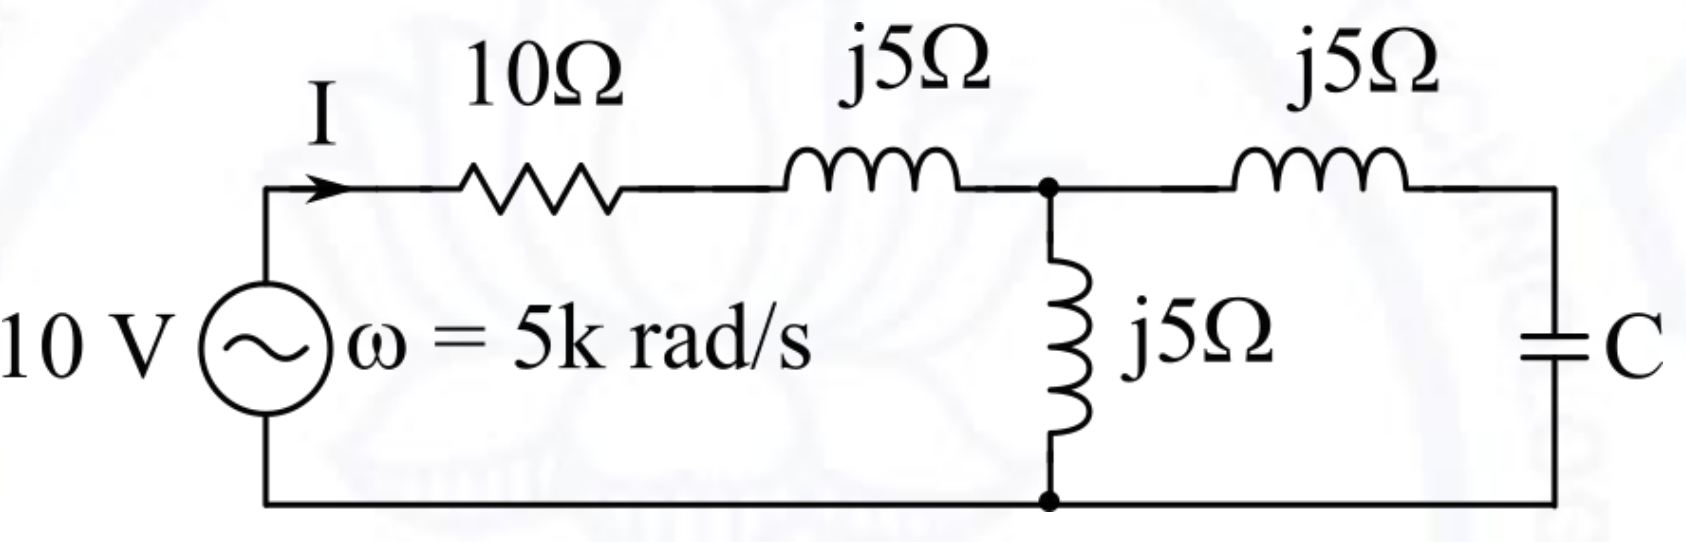
\includegraphics[width=1\linewidth]{2021/EE/14/figs/qf1.png}
\end{figure}\\
\textit{Solution:- }
\fi
\begin{table}[h!]
        \begin{tabular}{ | m{1.0cm} | m{1.5cm} |m{2.5cm} |} 
  \hline
 Symbol & Value &Description\\ 
 \hline
$C$& --&  capacitance \\
\hline
$X_L$&$\omega L=5 \ohm$& inductive reactance  \\
\hline
\end{tabular}\\
\label{rajmalt4gate21ee}
\caption{}
    
    \end{table}\\
Using Laplace transform , modified figure is 
\begin{figure}[h!]
   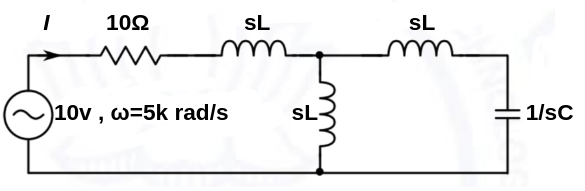
\includegraphics[width=1\linewidth]{2021/EE/14/figs/f2.png}
\end{figure}\\
For $I=0 $ , 
\begin{align}
Z & =\infty\\
    Z&=10+sL+\brak{\frac{\brak{sL+\frac{1}{sC}}\times sL}{sL+\frac{1}{sC}+ sL}}\\
&=10+sL+\frac{sL+\frac{1}{sC}}{1+\frac{1}{s^{2}LC}+1}
\end{align}
\begin{align}
 \implies   2+\frac{1}{s^{2}LC}&=0
\end{align}
\begin{align}
     C&=\frac{-1}{2s^2L}\\
       &=\frac{1}{2\brak{\omega L}\omega }\\
       \implies C&= 20\mu F
\end{align}

%\end{document}
